%%
%% This is file `template-8d.tex',
%% generated with the docstrip utility.
%%
%% The original source files were:
%%
%% template.raw  (with options: `8d')
%% 
%% Template for the LaTeX class aipproc.
%% 
%% (C) 1998,2000,2001 American Institute of Physics and Frank Mittelbach
%% All rights reserved
%% 
%%
%% $Id: template.raw,v 1.12 2005/07/06 19:22:14 frank Exp $
%%

%%%%%%%%%%%%%%%%%%%%%%%%%%%%%%%%%%%%%%%%%%%%
%% Please remove the next line of code if you
%% are satisfied that your installation is
%% complete and working.
%%
%% It is only there to help you in detecting
%% potential problems.
%%%%%%%%%%%%%%%%%%%%%%%%%%%%%%%%%%%%%%%%%%%%

%
% $Id: aipcheck.tex,v 1.9 2005/12/01 16:16:27 frank Exp $
%
%%%%%%%%%%%%%%%%%%%%%%%%%%%%%%%%%%%%%%%%%%%%%%%%%%
% Testing for potential problems with this class
%%%%%%%%%%%%%%%%%%%%%%%%%%%%%%%%%%%%%%%%%%%%%%%%%%

\newif\ifproblem
\newif\ifobservation
\newif\iftimesok

\makeatletter
\def\IfStandaloneCheck{\def\next{aipcheck}
  \edef\currjob{\jobname}
  \edef\next{\meaning\next}
  \edef\currjob{\meaning\currjob}
  \ifx\currjob\next
    \expandafter\@firstoftwo
  \else
    \expandafter\@secondoftwo
  \fi
}
\makeatother

\typeout{***********************************************}
\typeout{*}
\typeout{* Testing if all files required for the aipproc}
\typeout{* class are available ...}
\typeout{*}
\typeout{***********************************************}

\typeout{*}
\typeout{* Looking for LaTeX2e ... }
\ifx\documentclass\undefined
 \typeout{*}
 \typeout{* Sorry this is a fatal error:}
 \typeout{*}
 \typeout{* The aipproc class can only be used with LaTeX2e which is}
 \typeout{* the standard LaTeX since 1994!}
 \typeout{*}
 \typeout{* Please make sure that your version of LaTeX is up-to-date}
 \typeout{* before attempting to use this class.}
 \typeout{*}
 \expandafter\stop
\else
 \typeout{* ... ok }
\fi


\def\next#1/#2/#3\next{#1#2}
\typeout{*}
\typeout{* Testing that LaTeX2e is not too old ... }
\ifnum\expandafter\next\fmtversion\next<199612 \relax
 \typeout{* ... what a vintage! }
 \typeout{*}
 \typeout{* Sorry this is a fatal error:}
 \typeout{*}
 \typeout{* The aipproc class can only be used with a recent version}
 \typeout{* of LaTeX2e. Your version is dated \fmtversion\space --- but}
 \typeout{* at least the 1996/12/01 version is required!}
 \typeout{*}
 \typeout{* Please make sure that your version of LaTeX is up-to-date}
 \typeout{* before attempting to use this class.}
 \typeout{*}
 \expandafter\stop
\else
 \ifnum\expandafter\next\fmtversion\next<199806 \relax
   \typeout{* ... probably ok }
   \typeout{*}
   \typeout{* Your version of LaTeX2e is quite old --- the aipproc class}
   \typeout{* hasn't been tested with your release.}
   \typeout{*}
   \typeout{* We believe that it will probably work, but if you encounter}
   \typeout{* problems you will need upgrade your installation.}
   \typeout{*}
   \typein{* Type <return> to continue ...}
   \problemtrue
 \else
   \typeout{* ... ok }
 \fi
\fi


\typeout{*}
\typeout{* Looking for aipproc.cls ... }
\IfFileExists{aipproc.cls}
    {
     \typeout{* ... ok }
    }
    {
     \typeout{* ... not found! }
     \typeout{*}
     \typeout{* Sorry this is a fatal error:}
     \typeout{*}
     \typeout{* Before you can use the aipproc class you have to unpack}
     \typeout{* it from the documented source.}
     \typeout{*}
     \typeout{* Run LaTeX on the file 'aipproc.ins', e.g.,}
     \typeout{*}
     \typeout{* \space\space latex aipproc.ins}
     \typeout{*}
     \typeout{* or whatever is necessary on your installation to process}
     \typeout{* a file with LaTeX. This should unpack a number of files for you:}
     \typeout{*}
     \typeout{* aipproc.cls \space and \space aip-*.clo}
     \typeout{*}
     \typeout{* After that retry processing this guide.}
     \typeout{*}
     \stop
}

\typeout{*}
\typeout{* Looking for aipxfm.sty ... }
\IfFileExists{aipxfm.sty}
    {
     \typeout{* ... ok }
    }
    {
     \typeout{* ... not found! }
     \typeout{*}
     \typeout{* Sorry this is a fatal error:}
     \typeout{*}
     \typeout{* The aipxfm.sty file which is part of the aipproc distribution}
     \typeout{* must be installed in a directory which is searched by LaTeX.}
     \typeout{*}
     \typeout{* Please install this file and retry.}
     \typeout{*}
     \stop
}

\typeout{*}
\typeout{* Looking for aip-8s.clo ... }
\IfFileExists{aip-8s.clo}
    {
     \typeout{* ... ok }
    }
    {
     \typeout{* ... not found! }
     \typeout{*}
     \typeout{* Sorry this is a fatal error:}
     \typeout{*}
     \typeout{* The aip-8s.clo file which is part of the aipproc distribution}
     \typeout{* must be installed in a directory which is searched by LaTeX.}
     \typeout{*}
     \typeout{* Please install this file and retry.}
     \typeout{*}
     \stop
}

\typeout{*}
\typeout{* Looking for aip-8d.clo ... }
\IfFileExists{aip-8d.clo}
    {
     \typeout{* ... ok }
    }
    {
     \typeout{* ... not found! }
     \typeout{*}
     \typeout{* Sorry this is a fatal error:}
     \typeout{*}
     \typeout{* The aip-8d.clo file which is part of the aipproc distribution}
     \typeout{* must be installed in a directory which is searched by LaTeX.}
     \typeout{*}
     \typeout{* Please install this file and retry.}
     \typeout{*}
     \stop
}


\typeout{*}
\typeout{* Looking for aip-6s.clo ... }
\IfFileExists{aip-6s.clo}
    {
     \typeout{* ... ok }
    }
    {
     \typeout{* ... not found! }
     \typeout{*}
     \typeout{* Sorry this is a fatal error:}
     \typeout{*}
     \typeout{* The aip-6s.clo file which is part of the aipproc distribution}
     \typeout{* must be installed in a directory which is searched by LaTeX.}
     \typeout{*}
     \typeout{* Please install this file and retry.}
     \typeout{*}
     \stop
}


\iffalse
\typeout{*}
\typeout{* Looking for aip-arlo.clo ... }
\IfFileExists{aip-arlo.clo}
    {
     \typeout{* ... ok }
    }
    {
     \typeout{* ... not found! }
     \typeout{*}
     \typeout{* Sorry this is a fatal error:}
     \typeout{*}
     \typeout{* The aip-arlo.clo file which is part of the aipproc distribution}
     \typeout{* must be installed in a directory which is searched by LaTeX.}
     \typeout{*}
     \typeout{* Please install this file and retry.}
     \typeout{*}
     \stop
}
\fi

\typeout{*}
\typeout{* Looking for fixltx2e.sty ... }
\IfFileExists{fixltx2e.sty}
    {
     \typeout{* ... ok }
    }
    {
     \typeout{* ... not found, trying fix2col.sty instead ... }
     \typeout{*}
     \IfFileExists{fix2col.sty}
         {
          \typeout{* ... ok }
         }
         {
          \typeout{* ... not found! }
          \typeout{*}
          \typeout{* Sorry this is a fatal error:}
          \typeout{*}
          \typeout{* Your LaTeX distribution contains neither fixltx2e.sty}
          \typeout{* nor fix2col.sty.}
          \typeout{*}
          \typeout{* This means that it is either too old or incompletely}
          \typeout{* installed.}
          \typeout{*}
          \typeout{* fixltx2e.sty is part of the standard LaTeX distribution}
          \typeout{* since 1999; fix2col.sty is an earlier version of this}
          \typeout{* package.}
          \typeout{*}
          \typeout{* Best solution is to get the latest LaTeX distribution.}
          \typeout{* If this is impossible for you, download fix2col.sty.}
          \typeout{* You can get this software from a CTAN host.}
          \typeout{* Refer to http://www.ctan.org and search for "fix2col".}
          \typeout{*}
          \typeout{* After you have updated your LaTeX distribution}
          \typeout{* retry processing this guide.}
          \stop
     }
}

\typeout{*}
\typeout{* Looking for fontenc.sty ... }
\IfFileExists{fontenc.sty}
    {
     \typeout{* ... ok }
    }
    {
     \typeout{* ... not found! }
     \typeout{*}
     \typeout{* Sorry this is a fatal error:}
     \typeout{*}
     \typeout{* The fontenc package, which is part of standard LaTeX}
     \typeout{* (base distribution) has to be installed at the site to}
     \typeout{* run the aipproc class.}
     \typeout{*}
     \typeout{* The fact that it cannot be found either means that}
     \typeout{* this LaTeX release is too old or that it was installed}
     \typeout{* improperly.}
     \typeout{*}
     \typeout{* Please make sure that your version of LaTeX is okay}
     \typeout{* before attempting to use this class. The LaTeX distribution}
     \typeout{* contains the file "ltxcheck.tex" which can be used to}
     \typeout{* test the basic functionality and integrity of your installation.}
     \typeout{*}
     \stop
    }

\typeout{*}
\typeout{* Looking for calc.sty ... }
\IfFileExists{calc.sty}
    {
     \typeout{* ... ok }
    }
    {
     \typeout{* ... not found! }
     \typeout{*}
     \typeout{* Sorry this is a fatal error:}
     \typeout{*}
     \typeout{* The calc package, which is part of standard LaTeX}
     \typeout{* (tool distribution) has to be installed at the site}
     \typeout{* to run the aipproc class.}
     \typeout{*}
     \typeout{* The fact that it cannot be found either means that}
     \typeout{* this LaTeX release is too old or that it was installed}
     \typeout{* only in parts.}
     \typeout{*}
     \typeout{* Please make sure that the tools distribution of LaTeX}
     \typeout{* is installed before attempting to use this class.}
     \typeout{*}
     \typeout{* (You might be able to get calc.sty separately for your}
     \typeout{* installation if you are unable to upgrade to a recent}
     \typeout{* distribution for some reason.)}
     \typeout{*}
     \stop
    }

\typeout{*}
\typeout{* Looking for varioref.sty ... }
\IfFileExists{varioref.sty}
    {
     \typeout{* ... ok }
     \gdef\variorefoptionifavailable{varioref,}
    }
    {
     \typeout{* ... not found! }
     \typeout{*}
     \typeout{* Problem detected:}
     \typeout{*}
     \typeout{* The varioref package, which is part of standard LaTeX}
     \typeout{* (tool distribution) is not installed at this site.}
     \typeout{*}
     \typeout{* The fact that it cannot be found either means that}
     \typeout{* this LaTeX release is too old or that it was installed}
     \typeout{* only in parts.}
     \typeout{*}
     \typeout{* You can use the aipproc class without this package but }
     \typeout{* you cannot make use of the options "varioref" or "nonvarioref".}
     \typeout{*}
     \typeout{* Please also note that the aipguide.tex documentation}
     \typeout{* normally uses the "varioref" option to show its}
     \typeout{* effects (which  will now fail).}
     \typeout{*}
     \typein{* Type <return> to continue ...}
     \problemtrue
     \gdef\variorefoptionifavailable{}
     \let\vpageref\pageref
     \let\vref\ref
    }

\typeout{*}
\typeout{* Looking for times.sty ... }
\IfFileExists{times.sty}
    {
     \begingroup
% load times and forget it immediately again
       \RequirePackage{times}
       \global\expandafter\let\csname ver@times.sty\endcsname\relax    
       \long\def\next{ptm}
       \ifx\rmdefault\next
         \typeout{* ... ok }
         \gdef\psnfssproblemoption{}
         \endgroup
         \timesoktrue
       \else
         \endgroup
     \typeout{* ... obsolete! }
     \typeout{*}
     \typeout{* Serious problem detected:}
     \typeout{*}
     \typeout{* The times package, which is part of standard LaTeX}
     \typeout{* (psnfss distribution) is obsolete at this site.}
     \typeout{*}
     \typeout{* The fact that it contains incorrect code either means that}
     \typeout{* this LaTeX release is too old or that it was installed}
     \typeout{* only in parts with old files remaining!}
     \typeout{*}
     \typeout{* You can use the aipproc class without this package but}
     \typeout{* you have to specify the option "cmfonts" which result in}
     \typeout{* documents which are not conforming to the AIP layout specification!}
     \typeout{*}
     \typeout{* You can also try using the class in the following way:}
     \typeout{*}
     \typeout{* \space\space \string\documentclass[cmfonts]{aipproc}}
     \typeout{* \space\space \string\usepackage{times}}
     \typeout{* \space\space ...}
     \typeout{*}
     \typeout{* With luck this will result in Times Roman output but chances}
     \typeout{* are that you will get a larger number of error messages in}
     \typeout{* which case you have to remove the \string\usepackage declaration.}
     \typeout{*}
     \typein{* Type <return> to continue ...}
          \problemtrue
          \gdef\psnfssproblemoption{cmfonts}
          \def\textdegree{$^\circ$}            % used below but now
                                               % not setup
       \fi
    }
    {
     \typeout{* ... not found! }
     \typeout{*}
     \typeout{* Serious problem detected:}
     \typeout{*}
     \typeout{* The times package, which is part of standard LaTeX}
     \typeout{* (psnfss distribution) can not be found.}
     \typeout{*}
     \typeout{* The fact that this package cannot be found either means that}
     \typeout{* this LaTeX release is too old or that it was installed}
     \typeout{* only in parts!}
     \typeout{*}
     \typeout{* You can use the aipproc class without this package but }
     \typeout{* you have to specify the option "cmfonts" which result in}
     \typeout{* documents which are not conforming to the AIP layout specification!}
     \typeout{*}
     \typein{* Type <return> to continue ...}
     \problemtrue
     \gdef\psnfssproblemoption{cmfonts,}
    }

\iftimesok % don't bother testing other font options if times already
           % bad

\typeout{*}
\typeout{* Looking for t1ptm.fd or T1ptm.fd ... }
\IfFileExists{t1ptm.fd}
    {
     \typeout{* ... ok }
    }
    {
     \typeout{* ... not found, trying T1ptm.fd ... }
     \IfFileExists{T1ptm.fd}
          {
           \typeout{* ... ok }
          }
          {
           \typeout{* ... not found}
           \typeout{* Serious problem detected:}
           \typeout{*}
           \typeout{* The times package, which is part of standard LaTeX}
           \typeout{* (psnfss distribution) is available but the corresponding}
           \typeout{* .fd file (defining how to load Times Roman) is missing.}
           \typeout{*}
           \typeout{* The fact that this package is only partially installed}
           \typeout{* means that you LaTeX installation is unable to use Times}
           \typeout{* Roman fonts!}
           \typeout{*}
           \typeout{* You can use the aipproc class without this package but }
           \typeout{* you have to specify the option "cmfonts" which result in}
           \typeout{* documents which are not conforming to the AIP layout}
           \typeout{* specification!}
           \typeout{*}
           \typein{* Type <return> to continue ...}
           \problemtrue
           \timesokfalse
           \gdef\psnfssproblemoption{cmfonts,}
          }
    }

\fi


\newcommand\CheckFDFile[3]{%
  \typeout{*}
  \typeout{* Looking for #1#3.fd or #2#3.fd ... }
  \IfFileExists{#1#3.fd}
    {
     \typeout{* ... ok }
    }
    {
     \IfFileExists{#2#3.fd}
      {
       \typeout{* ... ok }
      }
      {\problemtrue
       \typeout{* ... not found! }
      }
    }
}

\iftimesok % don't bother testing other font options if Times already bad

%\CheckFDFile{ot1}{OT1}{ot1ztmcm}
%\CheckFDFile{oml}{OML}{omlztmcm}
%\CheckFDFile{oms}{OMS}{omsztmcm}
%\CheckFDFile{omx}{OMX}{omxztmcm}

\typeout{*}
\typeout{* Looking for mathptm.sty ... }
\IfFileExists{mathptm.sty}
    {
     \typeout{* ... ok }
     \CheckFDFile{ot1}{OT1}{ptmcm}
     \CheckFDFile{oml}{OML}{ptmcm}
     \CheckFDFile{oms}{OMS}{pzccm}
     \CheckFDFile{omx}{OMX}{psycm}
     \ifproblem
      \typeout{*}
      \typeout{* Problem detected:}
      \typeout{*}
      \typeout{* The mathptm package, which is part of standard LaTeX}
      \typeout{* (psnfss distribution) was found but some or all of its}
      \typeout{* support files describing which fonts to load are missing!}
      \typeout{*}
      \typeout{*}
      \typeout{* The fact that this package is only partially installed}
      \typeout{* means that the mathptm package cannot be used!}
      \typeout{*}
      \typeout{* You can use the aipproc class without this package but }
      \typeout{* you have to specify the option "nomathfonts" so that}
      \typeout{* math formulas will be typeset using Computer Modern.}
      \typeout{*}
      \typein{* Type <return> to continue ...}
      \problemtrue
      \gdef\psnfssproblemoption{nomathfonts,}
     \else
      \typeout{*}
      \typeout{* Looking for mathptmx.sty ... }
      \IfFileExists{mathptmx.sty}
       {
        \typeout{* ... ok }
        \CheckFDFile{ot1}{OT1}{ztmcm}
        \CheckFDFile{oml}{OML}{ztmcm}
        \CheckFDFile{oms}{OMS}{ztmcm}
        \CheckFDFile{omx}{OMX}{ztmcm}
        \ifproblem
          \typeout{*}
          \typeout{* Problem detected:}
          \typeout{*}
          \typeout{* The mathptmx package, which is part of standard LaTeX}
          \typeout{* (psnfss distribution) was found but some or all of its}
          \typeout{* support files describing which fonts to load are missing!}
          \typeout{*}
          \typeout{*}
          \typeout{* The fact that this package is only partially installed}
          \typeout{* means that the mathptmx package cannot be used!}
          \typeout{*}
          \typeout{* You can use the aipproc class without this package but }
          \typeout{* you have to specify the option "mathptm" (no x) so that}
          \typeout{* math formulas use the older version with upright greek letters.}
          \typeout{*}
          \typein{* Type <return> to continue ...}
          \problemtrue
          \gdef\psnfssproblemoption{mathptm,}
        \fi
       }
       {
        \typeout{* ... not found! }
        \typeout{*}
        \typeout{* Problem detected:}
        \typeout{*}
        \typeout{* The mathptmx package, which is part of standard LaTeX}
        \typeout{* (psnfss distribution) can not be found.}
        \typeout{*}
        \typeout{* This is unfortunate but not a disaster as the older}
        \typeout{* version of the package "mathptm" (no x) seems to exist.}
        \typeout{*}
        \typeout{* You can use the aipproc class without this package but }
        \typeout{* you have to specify the option "mathptm" so that}
        \typeout{* math formulas use the older version with upright greek letters.}
        \typeout{*}
        \typein{* Type <return> to continue ...}
        \problemtrue
        \gdef\psnfssproblemoption{mathptm,}
       }
      \fi
    }
    {
     \typeout{* ... not found! }
     \typeout{*}
     \typeout{* Problem detected:}
     \typeout{*}
     \typeout{* The mathptm package, which is part of standard LaTeX}
     \typeout{* (psnfss distribution) can not be found.}
     \typeout{*}
     \typeout{* The fact that this package cannot be found either means that}
     \typeout{* this LaTeX release is too old or that it was installed}
     \typeout{* only in parts!}
     \typeout{*}
     \typeout{* You can use the aipproc class without this package but }
     \typeout{* you have to specify the option "nomathfonts" so that}
     \typeout{* math formulas will be typeset using Computer Modern.}
     \typeout{*}
     \typein{* Type <return> to continue ...}
     \problemtrue
     \gdef\psnfssproblemoption{nomathfonts,}
    }

\typeout{*}
\typeout{* Looking for mathtime.sty ... }
\IfFileExists{mathtime.sty}
    {
     \typeout{* ... ok }
    }
    {
     \typeout{* ... not found! }
     \typeout{*}
     \typeout{* The mathime package can not be found.}
     \typeout{*}
     \typeout{* This is not a real problem but an observation,}
     \typeout{* because this package is only of interest}
     \typeout{* if you own the commerical MathTime fonts.}
     \typeout{*}
     \typeout{* You can use the aipproc class without this package but }
     \typeout{* you cannot use the "mathtime" option of the class.}
     \typeout{*}
     \observationtrue
    }
\typeout{*}
\typeout{* Looking for mtpro.sty ... }
\IfFileExists{mtpro.sty}
    {
     \typeout{* ... ok }
    }
    {
     \typeout{* ... not found! }
     \typeout{*}
     \typeout{* The mtpro package can not be found.}
     \typeout{*}
     \typeout{* This is not a real problem but an observation,}
     \typeout{* because this package is only of interest}
     \typeout{* if you own the commerical MathTime Professional fonts.}
     \typeout{*}
     \typeout{* You can use the aipproc class without this package but }
     \typeout{* you cannot use the "mtpro" option of the class.}
     \typeout{*}
     \observationtrue
    }
\else
\fi % iftimesok

\typeout{*}
\typeout{* Looking for graphicx.sty ... }
\IfFileExists{graphicx.sty}
    {
     \typeout{* ... ok }
    }
    {
     \typeout{* ... not found! }
     \typeout{*}
     \typeout{* Problem detected:}
     \typeout{*}
     \typeout{* The graphics package, which is part of standard LaTeX}
     \typeout{* (graphics distribution) can not be found.}
     \typeout{*}
     \typeout{* The fact that this package cannot be found either means that}
     \typeout{* this LaTeX release is too old or that it was installed}
     \typeout{* only in parts!}
     \typeout{*}
     \typeout{* You can use the aipproc class without this package but }
     \typeout{* you cannot use commands like \protect\includegraphics
                or \protect\resizebox}
     \typeout{* in this case.}
     \typeout{*}
     \typeout{* Please note that you will get a further error message below}
     \typeout{* about: "graphicx.sty not found" because the class will try}
     \typeout{* to load this package! Type return in response to that error.}
     \typeout{*}
     \typeout{* As a result the illustrations in aipguide will look strange.}
     \typeout{*}
     \typein{* Type <return> to continue ...}

     \gdef\resizebox##1##2{}
     \gdef\includegraphics{\textbf{graphics package missing:}}
     \problemtrue
    }

\typeout{*}
\typeout{* Looking for textcomp.sty ... }
\IfFileExists{textcomp.sty}
    {
     \typeout{* ... ok }
    }
    {
     \typeout{* ... not found! }
     \typeout{*}
     \typeout{* Problem detected:}
     \typeout{*}
     \typeout{* The textcomp package, which is part of standard LaTeX}
     \typeout{* (base distribution) can not be found.}
     \typeout{*}
     \typeout{* The fact that this package cannot be found either means that}
     \typeout{* this LaTeX release is too old or that it was installed}
     \typeout{* only in parts!}
     \typeout{*}
     \typeout{* You can use the aipproc class without this package but }
     \typeout{* you will always get the error: "textcomp.sty not found"}
     \typeout{* because the class will try to load this package!}
     \typeout{* Type return in response to that error.}
     \typeout{*}
     \typein{* Type <return> to continue ...}

     \def\textdegree{$^\circ$}         % used below but now
                                       % not set up
     \problemtrue
    }


\typeout{*}
\typeout{* Looking for url.sty ... }
\IfFileExists{url.sty}
    {
     \typeout{* ... ok }
    }
    {
     \typeout{* ... not found! }
     \typeout{*}
     \typeout{* Problem detected:}
     \typeout{*}
     \typeout{* The url package, which should be part of a good LaTeX}
     \typeout{* distribution, can not be found.}
     \typeout{*}
     \typeout{* Without this package you will not be able to use the \string\url}
     \typeout{* command. Try to download this package from a CTAN  host.}
     \typeout{* Refer to http://www.ctan.org and search for "url".}
     \typeout{*}
     \typein{* Type <return> to continue ...}

     \problemtrue
    }


\typeout{*}
\typeout{* Looking for textcase.sty ... }
\IfFileExists{textcase.sty}
    {
     \typeout{* ... ok }
    }
    {
     \typeout{* ... not found! }
     \typeout{*}
     \typeout{* Problem detected:}
     \typeout{*}
     \typeout{* The textcase package, which should be part of a good LaTeX}
     \typeout{* distribution, can not be found.}
     \typeout{*}
     \typeout{* Without this package you should be careful not to put math}
     \typeout{* formulas into \noexpand\section headings as these headings are}
     \typeout{* converted to UPPERCASE and might spoil your formulas.}
     \typeout{* Try to download this package from a CTAN  host.}
     \typeout{* Refer to http://www.ctan.org and search for "url".}
     \typeout{*}
     \typein{* Type <return> to continue ...}

     \problemtrue
    }


\makeatletter

\typeout{*}
\typeout{* Looking for natbib.sty ... }
\IfFileExists{natbib.sty}
    {
     \IfStandaloneCheck
       {\begingroup
        \let\@listi\relax
        \let\thebibliography\@empty
        \let\bibstyle\@empty
        \RequirePackage{natbib}
        \@ifpackagelater{natbib}{1999/05/29}
          {
           \typeout{* ... ok }
          }{
           \typeout{* ... might be too old! }
           \typeout{*}
           \typeout{* Your version of the natbib package might be too}
           \typeout{* old to be usable. This class was designed to}
           \typeout{* work with the version 7.0 dated 1999/05/28}
           \typeout{*}
           \typeout{* If problems occur download a}
           \typeout{* recent version from a CTAN host.}
           \typeout{*}
           \typeout{* Refer to http://www.ctan.org and search for "natbib".}
           \typeout{*}
           \typein{* Type <return> to continue ...}

           \global\problemtrue
          }
        \endgroup
        }{}
    }
    {
     \typeout{* ... not found! }
     \typeout{*}
     \typeout{* Serious problem detected:}
     \typeout{*}
     \typeout{* The natbib package, which should be part of a good LaTeX}
     \typeout{* distribution, can not be found.}
     \typeout{*}
     \typeout{* Without this package you will not be able to use certain}
     \typeout{* citation styles. See the aipguide documentation!}
     \typeout{*}
     \typeout{* Especially the layout for ARLO requires this package!}
     \typeout{*}
     \typeout{* Try to download this package from a CTAN  host.}
     \typeout{* Refer to http://www.ctan.org and search for "natbib".}
     \typeout{*}
     \typein{* Type <return> to continue ...}

     \problemtrue
    }

\makeatother


\typeout{*}
\typeout{* ... finished testing}
\typeout{*}
\ifproblem
\typeout{* The tests have revealed some problems in your TeX installation.}
\typeout{*}
\typeout{* Please review the above comments carefully and read the file}
\typeout{* README for further information.}
\typeout{*}
\typeout{*****************************************************************}
\typein{* Type <return> to continue ...}
\else
 \ifobservation
  \typeout{****************************************************************}
  \typeout{*}
  \typeout{* The tests have reveiled no problems in your TeX installation,}
  \typeout{* but some observations have been made; see above.}
  \typeout{*}
  \typeout{****************************************************************}
 \else
  \typeout{****************************************************************}
  \typeout{*}
  \typeout{* The tests have reveiled no problems in your TeX installation.}
  \typeout{*}
  \typeout{****************************************************************}
 \fi
\fi


% if this file is run standalone stop otherwise continue

\makeatletter
\IfStandaloneCheck
 {
\typeout{*}
\typeout{* This document only produces terminal output.}
\typeout{*}
\stop
 }
 {
\AtBeginDocument{\relax\ifx\xfm@address@loop\@undefined
  \typeout{***************************}
  \typeout{* Oooops ... you seem to have picked up an obsolete}
  \typeout{* aipproc.cls file from a previous installation!}
  \typeout{*}
  \typeout{* Please check that LaTeX finds the right one.}
  \typeout{*}
  \typeout{* Sorry have to give up ....}
  \typeout{***************************}
  \stop
 \fi}
 }
\makeatother

\endinput

%%% Local Variables: 
%%% mode: latex
%%% TeX-master: t
%%% End: 


%%%%%%%%%%%%%%%%%%%%%%%%%%%%%%%%%%%%%%%%%%%%
%% SELECT THE LAYOUT
%%
%% The class supports further options.
%% See aipguide.pdf for details.
%%
%%%%%%%%%%%%%%%%%%%%%%%%%%%%%%%%%%%%%%%%%%%%

\documentclass[
    ,final            % use final for the camera ready runs
%%  ,draft            % use draft while you are working on the paper
%%  ,numberedheadings % uncomment this option for numbered sections
%%  ,                 % add further options here if necessary
  ]
  {aipproc}

\layoutstyle{8x11double}

%%%%%%%%%%%%%%%%%%%%%%%%%%%%%%%%%%%%%%%%%%%%
%% FRONTMATTER
%%%%%%%%%%%%%%%%%%%%%%%%%%%%%%%%%%%%%%%%%%%%

\begin{document}

\title{Fixed Size Least Squares Support Vector Machines: Scalable Implementation for Large Scale Predictive Models}

\classification{<Replace this text with PACS numbers; choose from this list:
                \texttt{http://www.aip..org/pacs/index.html}>}
\keywords      {FS LSSVM, Big Data, Large Scale Models, Kernel SVM}

\author{Mandar Chandorkar}{
  address={<author1 address>}
}

\author{Oliver Lauwers}{
  address={<common address for author2 and author3>}
}

\author{Raghvendra Mall}{
  address={<common address for author2 and author3>}
  ,altaddress={<author1 address>} % additional visiting address
}

\author{Johann A.K Suykens}{
  address={<common address for author2 and author3>}
  ,altaddress={<author1 address>} % additional visiting address
}


\begin{abstract}
 This template file shows how to use the \texttt{aipproc} class to
 produce a paper with the correct layout for \emph{%
   AIP Conference Proceedings  8.5in x 11in double column}.

 A full description of the features supported by the \texttt{aipproc}
 class can be found in the \texttt{aipguide.pdf} document accompanying
 the distribution.

 Frequently asked questions can be found in the \texttt{FAQ.txt}
 document.
\end{abstract}

\maketitle

%%%%%%%%%%%%%%%%%%%%%%%%%%%%%%%%%%%%%%%%%%%%
%% MAINMATTER
%%%%%%%%%%%%%%%%%%%%%%%%%%%%%%%%%%%%%%%%%%%%

\section{<A section>}

  Infandum, regina, iubes renovare dolorem, Troianas ut opes et
  lamentabile regnum cruerint Danai; quaeque ipse miserrima vidi, et
  quorum pars magna fui. Quis talia fando Myrmidonum Dolopumve aut
  duri miles Ulixi temperet a lacrimis? Et iam nox umida caelo
  praecipitat, suadentque cadentia sidera somnos.

\section{<Another section>}

\subsection{<A subsection>}

Infandum, regina, iubes renovare dolorem, Troianas ut opes et
lamentabile\footnote{Here we test footnotes.} regnum cruerint Danai;
quaeque ipse miserrima vidi, et quorum pars magna fui. Quis talia
fando Myrmidonum Dolopumve aut duri miles Ulixi temperet a
lacrimis? Et iam nox umida caelo praecipitat, suadentque cadentia
sidera somnos. Sed si tantus amor casus cognoscere nostros
et\footnote{Et iam nox umida caelo praecipitat, suadentque cadentia
sidera somnos. Et iam nox umida caelo praecipitat, suadentque cadentia
sidera somnos.} breviter Troiae supremum audire laborem, quamquam
animus meminisse\footnote{Here we test footnotes.} horret, luctuque
refugit, incipiam.  Et iam nox umida caelo praecipitat, suadentque
cadentia sidera somnos. Sed si tantus amor casus
cognoscere\footnote{Here we test footnotes.} nostros et breviter Troiae
supremum audire laborem, quamquam animus meminisse horret,
luctuque refugit, incipiam.

Some url test \url{http://www.world.universe}.

\subsubsection{<A subsubsection>}

Et iam nox umida caelo praecipitat $J_{ion}$ suadentque cadentia
sidera somnos. Sed si tantus amor casus cognoscere nostros et breviter
Troiae $J_{ion}$ supremum audire laborem:
\begin{equation}
J_{ion}=A\frac{exp\left[-\frac{E_a}{kT}\right]}{kT}\alpha \label{ionflux}
\end{equation}
lamentabile regnum cruerint Danai; quaeque ipse miserrima vidi, et
quorum pars magna fui. $A$ talia fando, $E_a$ iam nox umida, $k$ caelo
praecipitat, suadentque cadentia sidera somnos. See \eqref{ionflux}.

\paragraph{<A subsubsubsection>}

Infandum, regina, iubes renovare dolorem, Troianas ut opes et
lamentabile regnum cruerint Danai; quaeque ipse miserrima vidi, et
quorum pars magna fui \cite{Brown2000,BrownAustin:2000}. Quis talia fando
Myrmidonum Dolopumve aut duri miles Ulixi temperet
\cite{Mittelbach/Schoepf:1990} a lacrimis? Et iam
nox umida caelo praecipitat, suadentque \cite{Wang} cadentia
sidera somnos.

%%%%%%%%%%%%%%%%%%%%%%%%%%%%%%%%%%%%%%%%%%%%
%% Sample figure:
%%
%% The option [height=...] scales the picture to the given height,
%% without it it would be printed at its nominal size
%%%%%%%%%%%%%%%%%%%%%%%%%%%%%%%%%%%%%%%%%%%%

\begin{figure}
  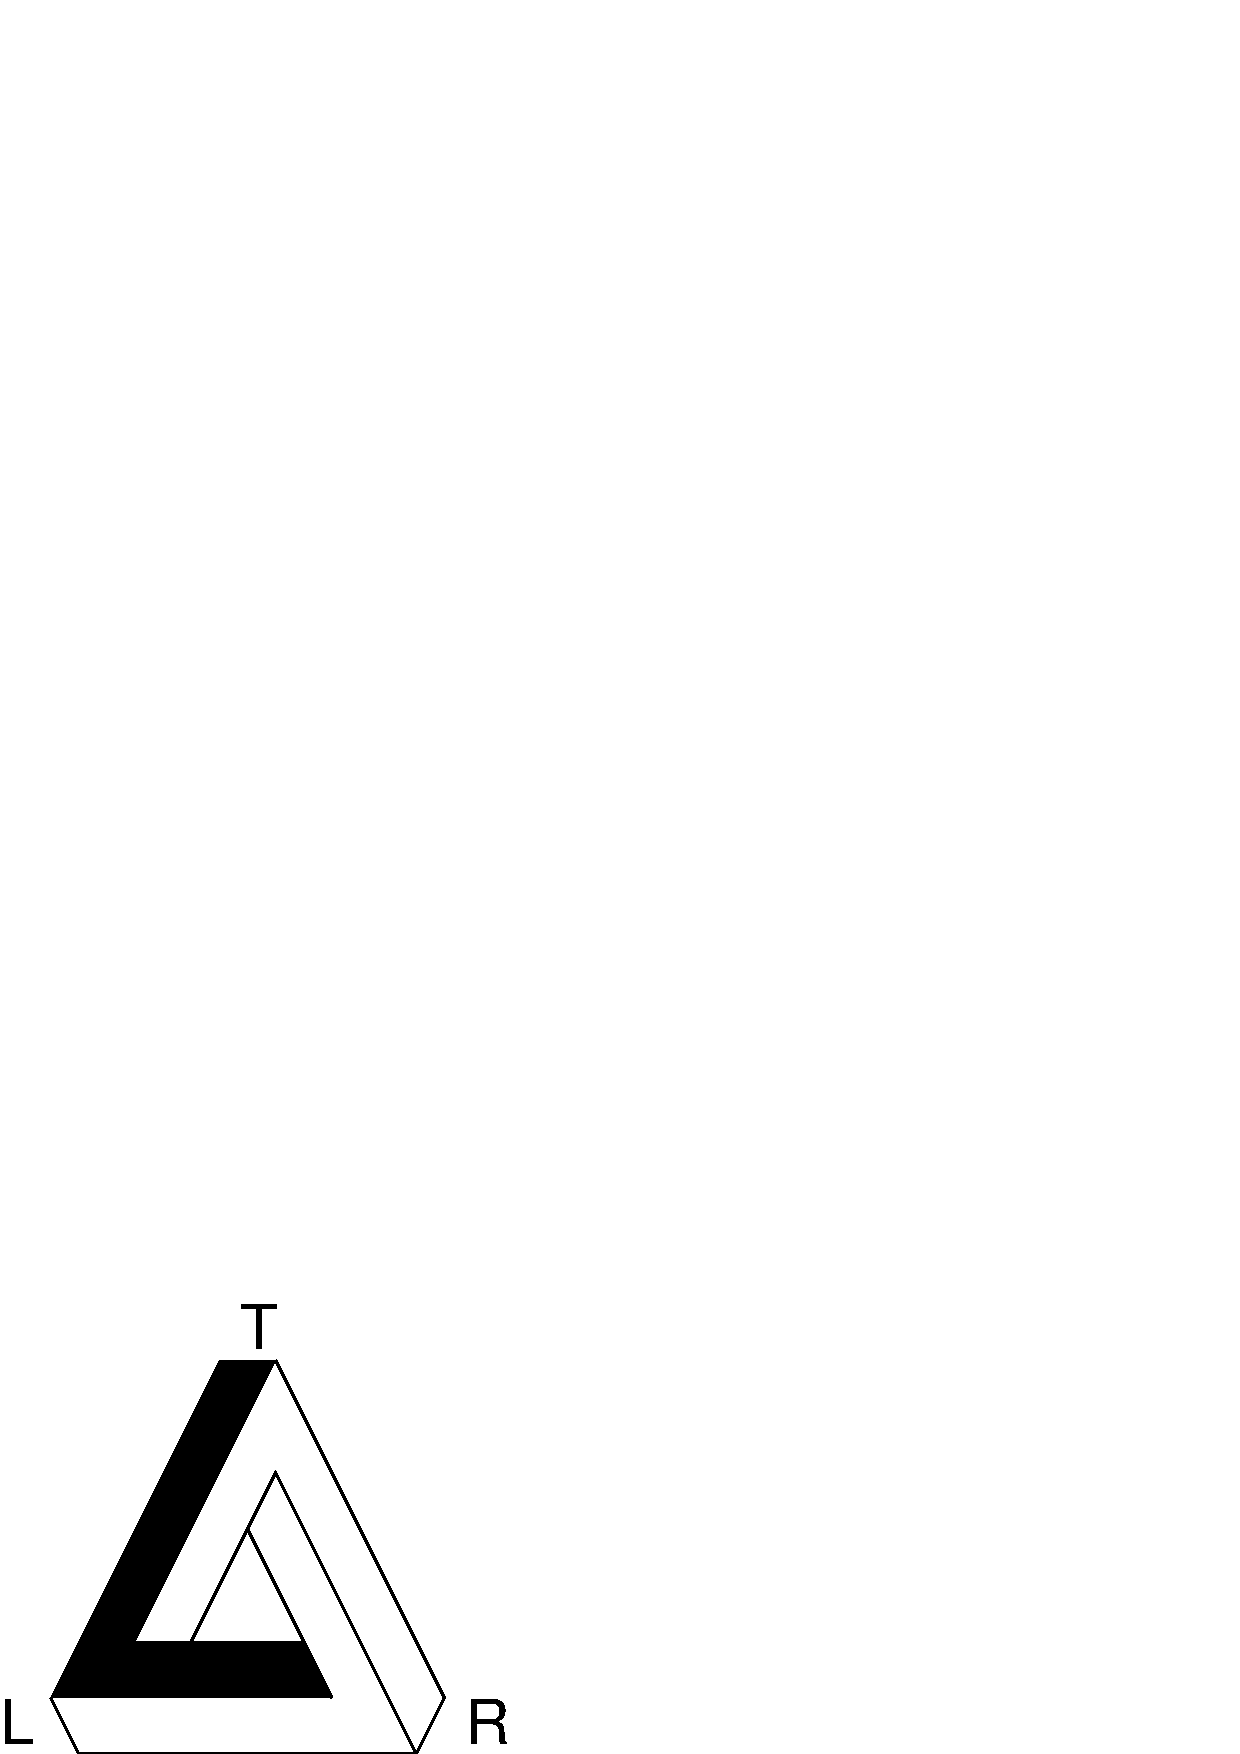
\includegraphics[height=.3\textheight]{escher}
  \caption{Picture to fixed height}
\end{figure}

Infandum, regina, iubes renovare dolorem, Troianas ut opes et
lamentabile regnum cruerint Danai; quaeque ipse miserrima vidi, et
quorum pars magna fui. Quis talia fando Myrmidonum Dolopumve aut duri
miles Ulixi temperet a lacrimis?

Infandum, regina, iubes renovare dolorem, Troianas ut opes et
lamentabile regnum cruerint Danai; quaeque ipse miserrima vidi, et
quorum pars magna fui. Quis talia\footnote{A few more footnotes} fando
Myrmidonum Dolopumve aut duri miles Ulixi temperet a lacrimis? Et iam
nox umida caelo praecipitat, suadentque cadentia\footnote{Here we test
footnotes.} sidera somnos. Sed si tantus amor casus cognoscere nostros
et breviter Troiae supremum audire laborem, quamquam animus meminisse
horret, luctuque refugit, incipiam.
In the following we test itemize environments up to the forth level.
\begin{itemize}
\item
  An item with more than a line of text. Infandum, regina, iubes
  renovare dolorem, Troianas ut opes et lamentabile regnum cruerint
  Danai.
\item
  Another item with sub entries
  \begin{itemize}
  \item
   A sub entry.
  \item
   Second sub entry.
    \begin{itemize}
    \item
     A sub sub entry.
      \begin{itemize}
      \item
       A sub sub sub entry.
      \item
       Second sub sub sub entry.
      \end{itemize}
    \item
     Second sub sub entry.
    \end{itemize}
  \end{itemize}
\item
  A final item.
\end{itemize}

%%%%%%%%%%%%%%%%%%%%%%%%%%%%%%%%%%%%%%%%%%%%
%% SAMPLE TABLE
%%
%% Shows the use of \tablehead and \tablenote
%% macros
%%%%%%%%%%%%%%%%%%%%%%%%%%%%%%%%%%%%%%%%%%%%

\begin{table}
\begin{tabular}{lrrrr}
\hline
  & \tablehead{1}{r}{b}{Single\\outlet}
  & \tablehead{1}{r}{b}{Small\tablenote{2-9 retail outlets}\\multiple}
  & \tablehead{1}{r}{b}{Large\\multiple}
  & \tablehead{1}{r}{b}{Total}   \\
\hline
1982 & 98 & 129 & 620    & 847\\
1987 & 138 & 176 & 1000  & 1314\\
1991 & 173 & 248 & 1230  & 1651\\
1998\tablenote{predicted} & 200 & 300 & 1500  & 2000\\
\hline
\end{tabular}
\caption{Average turnover per shop: by type
  of retail organisation}
\label{tab:a}
\end{table}

Infandum, regina, iubes renovare dolorem, Troianas ut opes et
lamentabile regnum cruerint Danai; quaeque ipse miserrima vidi, et
quorum pars magna fui. Quis talia fando Myrmidonum Dolopumve aut duri
miles Ulixi temperet a \cite{EVH:Office} lacrimis? In the following we
test enumrerate environments up to the second level. In addition we
look how ridiculous large labels look.
\begin{enumerate}
\item
  An item \cite{Liang:1983}
\item
  Another item with sub entries
  \begin{enumerate}
  \item
   A sub entry \cite{Wang}
  \item
   Second sub entry
  \end{enumerate}
\item
  The final item with normal label.
\end{enumerate}
Infandum, regina, iubes renovare dolorem, Troianas ut opes et
lamentabile regnum cruerint Danai; quaeque ipse miserrima vidi, et
quorum pars magna fui. Quis talia  fando Myrmidonum Dolopumve aut duri
miles Ulixi temperet a lacrimis?
\begin{description}
\item[Infandum]
 regina, iubes renovare dolorem, Troianas ut opes et lamentabile
 regnum cruerint Danai.
\item[Sed]
 si tantus amor casus cognoscere nostros et breviter Troiae supremum
 audire laborem, quamquam animus meminisse horret, luctuque refugit,
 incipiam.
\item[Lamentabile] regnum cruerint Danai; quaeque ipse miserrima vidi, et
quorum pars magna fui. Quis talia  fando Myrmidonum Dolopumve aut duri
miles Ulixi temperet a lacrimis?
\end{description}

Infandum, regina, iubes renovare dolorem, Troianas ut opes et
lamentabile regnum cruerint Danai; quaeque ipse miserrima vidi, et
quorum pars magna fui. Quis talia fando Myrmidonum Dolopumve aut duri
miles Ulixi temperet a lacrimis?
Infandum, regina, iubes renovare dolorem, Troianas ut opes et
lamentabile regnum cruerint Danai; quaeque ipse miserrima vidi, et
quorum pars magna fui. Quis talia fando Myrmidonum Dolopumve aut duri
miles Ulixi temperet a lacrimis?

Infandum, regina, iubes renovare dolorem, Troianas ut opes et
lamentabile regnum cruerint Danai; quaeque ipse miserrima vidi, et
quorum pars magna fui. Quis talia fando Myrmidonum Dolopumve aut duri
miles Ulixi temperet a lacrimis? Et iam nox umida caelo praecipitat,
suadentque cadentia sidera somnos. Sed si tantus amor casus
\cite{Liang:1983} cognoscere nostros et breviter Troiae supremum
audire laborem, quamquam animus meminisse horret, luctuque refugit,
incipiam.  Infandum, regina, iubes renovare dolorem, Troianas ut opes
et lamentabile regnum cruerint Danai; quaeque ipse miserrima vidi, et
quorum pars magna fui. Quis talia fando Myrmidonum Dolopumve aut duri
miles Ulixi temperet a \cite{SJ:1999} lacrimis? Et iam nox umida caelo
praecipitat, suadentque cadentia sidera somnos. Sed si tantus amor
casus cognoscere nostros et breviter Troiae supremum audire laborem,
quamquam animus meminisse horret, luctuque refugit, incipiam.

\section{<A section>}

Infandum, regina, iubes renovare dolorem, Troianas ut opes et
lamentabile regnum cruerint Danai; quaeque ipse miserrima vidi, et
quorum pars magna fui. Quis talia fando Myrmidonum Dolopumve aut duri
miles Ulixi temperet a lacrimis?

Et iam nox umida caelo praecipitat, suadentque cadentia sidera
somnos. Sed si tantus amor casus cognoscere nostros et breviter Troiae
supremum audire \cite{Knuth:WEB} laborem, quamquam animus meminisse
horret, luctuque refugitum, refugit, incipitat, suadenovare dolorem,
Troianas ut opes Ulixi temperet breviter Troiaeque ipse nostros et a
lacrimis?

Infandum, regina, iubes renovare dolorem, Troianas ut opes et
lamentabile regnum cruerint \cite{BrownAustin:2000} Danai; quaeque ipse
miserrima vidi, et quorum pars magna fui. Quis talia fando Myrmidonum
Dolopumve aut duri miles Ulixi temperet a lacrimis?  Infandum, regina,
iubes renovare dolorem, Troianas ut opes et lamentabile regnum
cruerint Danai; quaeque ipse miserrima vidi, et quorum pars magna
fui. Quis talia fando Myrmidonum Dolopumve aut duri miles Ulixi
temperet a lacrimis?

%%%%%%%%%%%%%%%%%%%%%%%%%%%%%%%%%%%%%%%%%%%%%%%%
%% BACKMATTER
%%%%%%%%%%%%%%%%%%%%%%%%%%%%%%%%%%%%%%%%%%%%%%%%

\begin{theacknowledgments}
  Infandum, regina, iubes renovare dolorem, Troianas ut opes et
  lamentabile regnum cruerint Danai; quaeque ipse miserrima vidi, et
  quorum pars magna fui. Quis talia fando Myrmidonum Dolopumve aut duri
  miles Ulixi temperet a lacrimis?
\end{theacknowledgments}

%%%%%%%%%%%%%%%%%%%%%%%%%%%%%%%%%%%%%%%%%%%%%%%%
%% The bibliography can be prepared using the BibTeX program or
%% manually.
%%
%% The code below assumes that BibTeX is used.  If the bibliography is
%% produced without BibTeX comment out the following lines and see the
%% aipguide.pdf for further information.
%%
%% For your convenience a manually coded example is appended
%% after the \end{document}
%%%%%%%%%%%%%%%%%%%%%%%%%%%%%%%%%%%%%%%%%%%%%%%%

%%%%%%%%%%%%%%%%%%%%%%%%%%%%%%%%%%%%%%%%%%%%%%%%
%% You may have to change the BibTeX style below, depending on your
%% setup or preferences.
%%
%%
%% For The AIP proceedings layouts use either
%%%%%%%%%%%%%%%%%%%%%%%%%%%%%%%%%%%%%%%%%%%%

\bibliographystyle{aipproc}   % if natbib is available
%\bibliographystyle{aipprocl} % if natbib is missing

%%%%%%%%%%%%%%%%%%%%%%%%%%%%%%%%%%%%%%%%%%%
%% You probably want to use your own bibtex database here
%%%%%%%%%%%%%%%%%%%%%%%%%%%%%%%%%%%%%%%%%%%
\bibliography{sample}

%%%%%%%%%%%%%%%%%%%%%%%%%%%%%%%%%%%%%%%%%%%
%% Just a reminder that you may have to run bibtex
%% All of it up to \end{document} can be removed
%% if you don't like the warning.
%%%%%%%%%%%%%%%%%%%%%%%%%%%%%%%%%%%%%%%%%%%
\IfFileExists{\jobname.bbl}{}
 {\typeout{}
  \typeout{******************************************}
  \typeout{** Please run "bibtex \jobname" to optain}
  \typeout{** the bibliography and then re-run LaTeX}
  \typeout{** twice to fix the references!}
  \typeout{******************************************}
  \typeout{}
 }

\end{document}

%%%%%%%%%%%%%%%%%%%%%%%%%%%%%%%%%%%%%%%%%%%
%% The following lines show an example how to produce a bibliography
%% without the help of the BibTeX program. This could be used instead
%% of the above.
%%%%%%%%%%%%%%%%%%%%%%%%%%%%%%%%%%%%%%%%%%%

\begin{thebibliography}{9}

\bibitem{Brown2000}
M.~P. Brown,  and K.~Austin, \emph{The New Physique}, Publisher Name,
  Publisher City, 2000, pp. 212--213.

\bibitem{BrownAustin:2000}
M.~P. Brown,  and K.~Austin, \emph{Appl. Phys. Letters} \textbf{85},
  2503--2504 (2000).

\bibitem{Wang}
R.~Wang, ``Title of Chapter,'' in \emph{Classic Physiques}, edited by
  R.~B. Hamil, Publisher Name, Publisher City, 2000, pp. 212--213.

\bibitem{SJ:1999}
C.~D.~Smith and E.~F.~Jones,  ``Load-Cycling in Cubic Press,'' in
  \emph{Shock Compression of Condensed Matter-1999}, edited by M.~D.~F. et~al.,
  AIP Conference Proceedings 505, American Institute of Physics, New York,
  1999, pp. 651--654.

\end{thebibliography}

\endinput
%%
%% End of file `template-8d.tex'.
